\section{Question 9}
\subsection{Part a}
\begin{figure}[H]
    \centering
    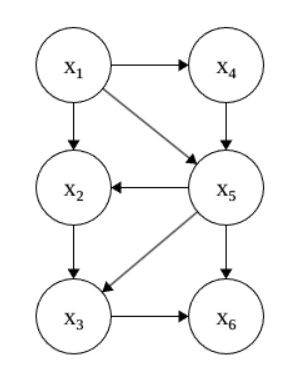
\includegraphics[width=0.3\textwidth]{../images/BN_Q9.png}  
\end{figure}
Justification: We use the algorithm for constructing an I-map of a given distribution given in Algorithm 3.2 of Friedman-Koller.\\
When $x_5$ is inserted, it has of course to be connected with $x_4$, but $x_1$ is also not independent of $x_5$ given $x_4$ in H. For $x_2$, $x_5$ and $x_1$ together separate it from $x_4$, and this blanket is minimal since it has to be connected to both $x_1$ and $x_5$. For $x_3$, $x_2$ is necessarily its parent. $x_3$ cannot be rendered independent of $x_5$ by any subset of $\{x_1, x_2, x_4\}$, so $x_5$ is also a parent. At this point, $x_3$ is separated from $x_1$ and $x_4$. For $x_6$, it is necessary to add its neighbours in H as its parents in G, and these d-separate it in H from all other vertices, so we are done.
In total, this approach created 9 directed edges.

\subsection{Part b}
A simple change that generates more variables is to consider the order $x_1, x_4, x_3, x_2, x_5, x_6$.
\begin{figure}[H]
    \centering
    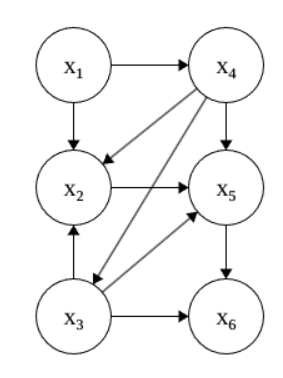
\includegraphics[width=0.3\textwidth]{../images/BN_Q9_2.png}
\end{figure}
When $x_3$ is inserted, no subset of $\{x_4, x_1\}$ d-separates it from the other vertex. When $x_2$ is now added, in the absence of $x_5$, it cannot be d-separated from $x_4$ by $x_1, x_3$ (note that due to monotonicity of d-separation in Markov networks, we do not need to separately consider subsets of $\{x_1, x_3\}$). $x_5$ needs to be connected with both its neighbours, and also with $x_3$ since $\{x_2, x_4\}$ does not d-separate it from $x_3$. $x_6$ has to be connected to all its neighbours, who form a Markov blanket.\\
In total, this approach created 10 directed edges.

\subsection{Part c}
$x_3 \independent x_5 | x_2, x_6$ and $x_5 \independent x_1 | x_2, x_4$ are two CIs that hold in H but not in G (since $x_3$ and $x_5$, $x_5$ and $x_1$ now have edges between them in G, but were d-separated from each other by an appropriate set of vertices in H).\\